\documentclass[11pt, a4paper]{article}

\usepackage[utf8]{inputenc}
\usepackage{authblk}
\usepackage{titlesec}

% Maths tools
\usepackage[tbtags]{amsmath}
\usepackage{amssymb}

% Margin
\usepackage[margin=2.9cm]{geometry}

% Line numbers
\usepackage{lineno}

%Scientific notation
\usepackage{siunitx}

% Landscape page
\usepackage{pdflscape}
\usepackage{afterpage}

% Spacing
\usepackage{setspace}
\doublespacing

% Enumeration
\usepackage{enumerate}

% indentation
\setlength\parindent{10pt}
\setlength{\parskip}{5pt}

% Figures
\usepackage{graphicx}
\usepackage{caption}
\usepackage{subcaption}
\usepackage{epstopdf}
\renewcommand{\thefigure}{\textbf{\arabic{figure}}}
\renewcommand{\figurename}{\textbf{Supplementary Figure}}

%table
\usepackage{multirow}
\usepackage{hhline}
\usepackage[table]{xcolor}
\renewcommand{\thetable}{\textbf{\arabic{table}}}
\renewcommand{\tablename}{\textbf{Supplementary Table}}

%footnotes
\usepackage{footmisc}
\renewcommand{\thefootnote}{\fnsymbol{footnote}}

% References
\usepackage[sort&compress, numbers,super]{natbib}
\bibliographystyle{unsrtnat}
\PassOptionsToPackage{hyphens}{url}\usepackage[colorlinks=true,linkcolor=magenta, citecolor=magenta]{hyperref}
\renewcommand\refname{Supplementary References}

%subsubsection format
\titleformat*{\subsubsection}{\large\it}

%highlighting text
\usepackage{color, xcolor,soul}
\definecolor{blau}{RGB}{236,226,240}
\soulregister\cite7
\soulregister\citet7
\soulregister\citealt7
\soulregister\citenum7
\soulregister\citep7
\soulregister\ref7
\DeclareRobustCommand{\hlc}[1]{{\sethlcolor{blau}\hl{#1}}}

\usepackage{makecell}

\usepackage{titlesec}% http://ctan.org/pkg/titlesec
\titleformat{\section}%
  [hang]% <shape>
  {\normalfont\bfseries\Large}% <format>
  {}% <label>
  {0pt}% <sep>
  {}% <before code>
  
\renewcommand{\thesection}{}% Remove section references...
\renewcommand{\thesubsection}{}%... from subsections
  \renewcommand{\thesubsubsection}{Supplementary Method \arabic{subsubsection}:}%... from subsections

\renewcommand{\arraystretch}{1.3}
  
%Title paper
\title{\vspace{-1cm} \normalsize Supplementary Information\\\vspace{0.2cm}
\LARGE Basic aspects of species' distributions}

\author{\textit{Bramon Mora et.\,al.}}

\date{}

\begin{document}
\maketitle
\thispagestyle{empty}

\clearpage

% Full description of Binomial model with multiple environmental covariates
% Full description of Categorical model with multiple environmental covariates
% Full description of Categorical model with heavy-tails---generalized error distribution
% Full description of Categorical model with heavy-tails---Student's t-distribution
% Full description of Categorical model with skewed---skewed normal distribution
% Using a MMSBM to calculate species similarity
% Edge problem in stan and need to define minimum probability.

\section*{Supplementary Methods}
\subsubsection*{Full description of the baseline model}
While the baseline model described in the main text included only one predictor, the same model can be extended to include multiple environmental variables. For example, imagine that we had $k$ predictors describing the environmental conditions of any given site $j$. The baseline model in Eq.~(1) of the main text could then be rewritten as:
\begin{equation}
\begin{split}
y_{ij} & \sim \text{Binomial}\left(1, p_{ij}\right) \\
\text{log}\left(p_{ij}\right) & = -\alpha_{i} - \sum_k \gamma_{ik} \left(x_{jk}-\beta_{ik}\right)^2,
\end{split}
\label{eq:baseline-binary}
\end{equation}
where $y_ij$ describes the presence and absence of species, and the prior distributions for the different parameters are analogous to the ones described in the main text.

Similarly, if the response variable $y_ij$ represented ordinal data (e.g.~Braun-Blanquet abundance-dominance classes), characterized by $K$ different classes. Then, one can adapt Supplementary Eq.~(\ref{eq:baseline-binary}) as:
\begin{equation}
\begin{split}
y_{ij} & \sim \text{Categorical}\left(\mathbf{q}\right) \\
q_{1} & = 1- p_{ij}\phi_1 \\
q_{k} & =  p_{ij}\phi_{k-1} -  p_{ij}\phi_{k} \\
q_{K} & =  p_{ij}\phi_{K-1} \\
\text{log}\left(p_{ij}\right) & = -\alpha_{i} - \sum_k \gamma_{ik} \left(x_{jk}-\beta_{ik}\right)^2 \\
\phi_1 & = \hat{\phi_1} \\
\phi_k & = \hat{\phi_k} \,\, \hat{\phi_{k-1}} \\
\hat{\phi} & = \text{Beta}(1,1),
\end{split}
\label{eq:baseline-categorical}
\end{equation}
where the prior distributions for the rest of parameters are analogous to the ones described in the main text.

\subsubsection*{Distance matrices from incomplete categorical and ordinal data}
The prior information that we have regarding species' distributions is represented by the set of ordinal and categorical traits found in the floristic database. More specifically, both the ecological indicator values and range of variation are ordinal traits, containing potential missing entries (Supplementary Table \ref{stab:EI}). These data could be directly used as covariates in any given distribution model; however, we want this information to be accounted for as a prior for the relevant parameters of our Bayesian model. One way to do so is by compiling the traits in the floristic database into variance-covariance matrices characterizing the \textit{a priori} similarity between species. To accomplish this, we need to turn the set of ecological indicator values and range of variation into the distance matrices $D$ presented in the text.
%, whereas plants' physiological data are characterized by categorical data containing multiple missing entries.

More generally, we want to understand the way $N$ species are characterized by $M$ categorical traits. One way to frame this problem is by using a network representation. Following the ideas presented by \citet{godoy-loriteAccurateScalableSocial2016}, we assume that species can be connected to each of these traits by an interaction $\left(i, j\right)$ that can be of any type $r\in R$. Notice that this provides us with multiple ways to account for the information---and lack thereof---contained in the different ordinal traits $M$. That is, the $R$ types of interactions can represent the lack of information for a particular link $\left(i, j\right)$, the absence or presence of such interaction, and any type of association between $i$ and $j$. Then, given a set of interactions $R^{*}$ between $N$ and $M$, we can use a Mixed Membership Stochastic Block Model (MMSBM) to understand the differences between species. In particular, these models consider that the $N$ plants and $M$ traits can be classified into $K$ and $L$ groups types, respectively. Then, they estimate `group-membership vectors', describing the extend to which the different plants and traits belong to the different group types.

Here, we use the MMSBM presented by \citet{godoy-loriteAccurateScalableSocial2016}, and classify plants into 5 types of species, and traits into 5 trait groups. Then, we estimate the group-membership vectors $\vec{\theta}_{\text{plants}}$, and calculate the pairwise distances $D_{ij}$ between plants as the euclidean distance between their membership vectors.  We run these models independently for species' ecological indicator values and their range of variation (Supplementary Table \ref{stab:EI}) to generate the two distance matrices for parameters $\beta_i$ and $\gamma_i$. Notice that the MMSBM uses an expectation-maximization algorithm to estimate the different membership vectors. Therefore, in order to have good estimates of the different pairwise distances $D_{ij}$ for $\beta_i$ and $\gamma_i$, one needs to run the MMSBM several times (1000 times) and average the resulting pairwise distances \citep{godoy-loriteAccurateScalableSocial2016, tarres-deulofeuTensorialBipartiteBlock2019}. 

This type of classification of ordinal variables that describe different species can also be done with other algorithms, including categorical PCA and matrix factorization methods. However, the MMSBM provides a convenient tool to classify very different types of traits, including categorical variables or diverse data containing multiple missing entries. Moreover, MMSBM have been shown to better capture the patterns of this sort of data \citet{godoy-loriteAccurateScalableSocial2016}.

%Given a set of interactions $R^{*}$ between $N$ and $M$, we use a Mixed Membership Stochastic Block Model (MMSBM) to characterize these. In particular, we consider that plants and traits can be classified into $K$ and $L$ groups, respectively. For every species $i$, we assume that there is a probability $\theta_{i\alpha}$ for it to belong to any of the $K$ species groups. Likewise, we also assume that any trait $j$ has a probability $\phi_{j\beta}$ of belonging to any of the $L$ trait groups. Finally, we define $p_{\alpha\beta}\left(r\right)$ as the probability of a species from group $\alpha$ interacting with a trait from group $\beta$ by an association type $r$. Putting these together, the probability of an interaction $\left(i, j\right)$ of type $r$ can be calculated as:
%\begin{equation}
%Pr[r_{ij}=r] = \sum_{\alpha \beta} \theta_{i\alpha} \phi_{j\beta} p_{\alpha\beta}\left(r\right)
%\end{equation}
%Following this definition, we want to find the group memberships that maximize the likelihood $P\left(R^{*}|\theta, \phi, p\right)$. Doing so is difficult optimization problem; however, it has been shown that one can estimate the different $\theta_{i\alpha}$, $\phi_{j\beta}$, and $p_{\alpha\beta}\left(r\right)$ parameters by maximizing the likelihood using an expectation-maximization algorithm \citep{godoy-loriteAccurateScalableSocial2016, tarres-deulofeuTensorialBipartiteBlock2019}. In simple terms, one can iteratively find multiple local minima for the likelihood, and average over the estimated the parameter values \citep{godoy-loriteAccurateScalableSocial2016}\footnote[2]{
%While this averaging is trivial for the estimated probabilities $Pr[r_{ij}=r]$, it is non-trivial if one wants to find averages for the group memberships. The reason for this is related to the stochastic nature of the expectation-maximization algorithm. This algorithm initially assigns random group memberships to both species and traits. While this random labelling is irrelevant when studying the probabilities $Pr[r_{ij}=r]$, it is instead crucial for averaging $\theta_{i\alpha}$, $\phi_{j\beta}$, and $p_{\alpha\beta}\left(r\right)$. Therefore, before averaging the group membership estimates, one needs to find the bijective relationship for the labellings of different iterations of the optimization algorithm. In a nutshell, for every iteration, I do this by using a simulated annealing algorithm on the estimated $p_{\alpha\beta}\left(r\right)$, matching the corresponding labelling to a reference iteration.}. 

%The average estimates for the group memberships provide us with a different scale to classify species based on the traits these have. In short, for any species $i$, we can estimate a $K$-dimensional vector $\vec{\theta}_{i}$ that describes the extend to which $i$ belong to each group membership---i.e. the extend to which a species is of one type or another. This classification is useful because it can be used to compare species, defining a way to measure the distance between species based on an arbitrary---and potentially incomplete---set of categorical or ordinal traits $M$. The simplest case is to define the distance as $D_{ij} = |\vec{\theta}_{i}-\vec{\theta}_{j}|$. Alternatively, one could also define $K$ distance matrices based on the different group memberships $D^{\alpha}_{ij} = |\theta_{i\alpha}-\theta_{j\alpha}|$.

%\subsubsection*{Sampling the posterior: simulated data and additional information}
%A good way to understand the model behaviour and the choice of prior distributions is by using simulated data. Here, we only present the simulations for the baseline model---the simplest model---but similar simulations were done for the others (see Code Availability section of the main text). 
%
%To simulate the data, we first generated two distance matrices relating the different parameters

\subsubsection*{Alternative variance-covariance structures}
The model structure defined above allows us to test how different sources of information characterize each of the different parameters. Specifically, we can do this by modifying Eq.~(\ref{eq:covariance-baseline}). For example, imagine that we have multiple matrices $D^k$ characterizing species' differences along different axis of variation---e.g.~two matrices characterizing physiological and environmental traits. One can modify Eq.~(\ref{eq:covariance-baseline}) for a particular parameter---e.g.~$\beta_{i}$---such that
\begin{equation} 
\Sigma_{ij} = \eta\,\text{exp}\left(-\sum_k\rho_{k} {D^{k}_{ij}}^2\right) + \delta_{ij} \sigma ,
\label{eq:covariance-complex}
\end{equation}
where now $\rho_{k}$ are separate relevance hyperparameters for each distance matrix in the total variance of $\beta_i$.

\section*{Supplementary Notes}
\section*{Supplementary Figures}

\begin{figure}[ht]
  \centering
    \vspace{0.5cm}
    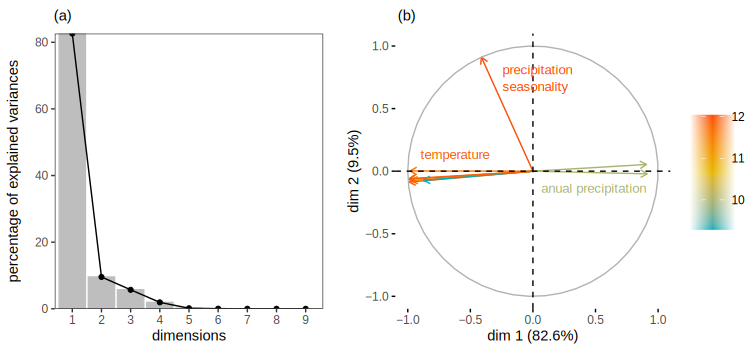
\includegraphics[width=1\textwidth]{figures/variances}
    	  \vspace{0.3cm}
	   \caption{PCA and variance explained.}
      \label{sfig:pca}
\end{figure}

\clearpage

%\begin{figure}[ht]
%  \centering
%    \vspace{0.5cm}
%    \includegraphics[width=1\textwidth]{figures/prior}
%    	  \vspace{0.3cm}
%	   \caption{Study of the priors for the baseline model presented in the main text.}
%     \label{sfig:sensitivity}
%\end{figure}
%\clearpage

\begin{figure}[ht]
  \centering
    \vspace{0.5cm}
    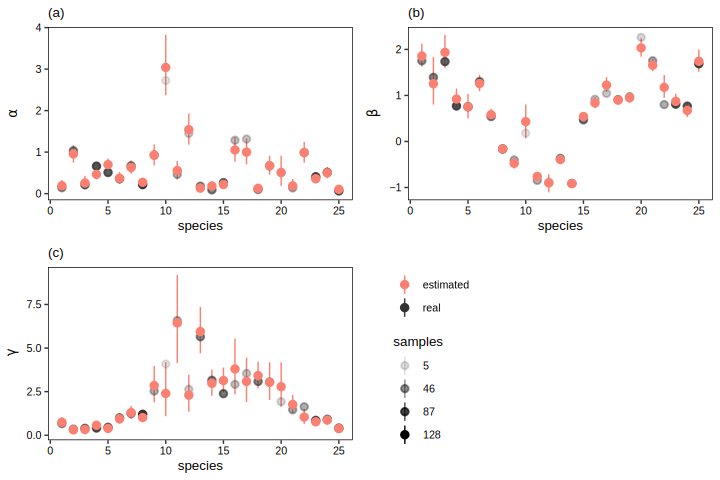
\includegraphics[width=1\textwidth]{figures/simulations-comparison}
    	  \vspace{0.3cm}
	   \caption{Studying the simulations. Transparency is a way to indicate the different sample sizes. Say that for both $\beta$ and $gamma$, the posterior distributions for the different species are correlated so that the variance between species increases as they are further apart.}
      \label{sfig:simulations}
\end{figure}

\clearpage

\begin{figure}[ht]
  \centering
    \vspace{0.5cm}
    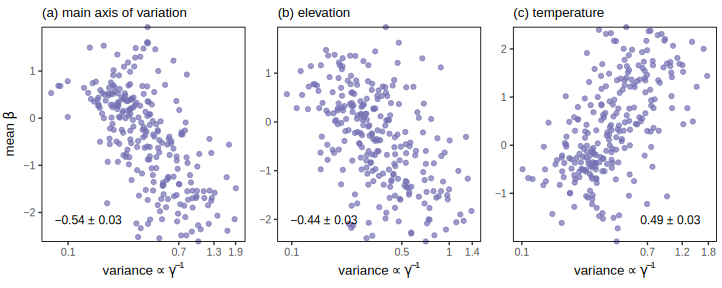
\includegraphics[width=1\textwidth]{figures/pca-elevation-temperature}
    	  \vspace{0.3cm}
	   \caption{The same as in Fig.~1 but with elevation and temperature.}
      \label{sfig:temperature-elevation}
\end{figure}

\clearpage

\begin{figure}[h]
  \centering
    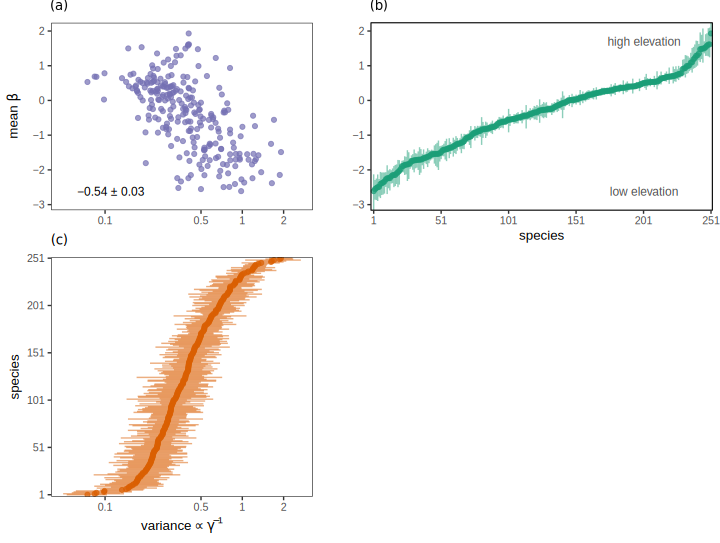
\includegraphics[width=0.9\textwidth]{figures/categorical-figure1}
    	  \vspace{0.1cm}
	   \caption{Universality of the relationship between mean and variance of species' distributions. Comparison between how different types of species are mapped in Fig.~\ref{fig:correlation}a. Panel (a) describes the correlation coefficient between $\beta_i$ and $\gamma_i$ for each type of species. Panel (b) shows the differences between neophytes and native species in the way these are distributed along the environmental gradient. Panel (c) shows the same differences for species that have decreased, decreased in low elevations, increase and remain stable over the last decades (see Supplementary Table 1 for further details).}
	   %7.5-4
      \label{sfig:categorical-baseline}
\end{figure}

\clearpage

\begin{figure}[h]
  \centering
    \vspace{0.5cm}
    \includegraphics[width=1\textwidth]{figures/figure1-secondaxis}
    	  \vspace{0.3cm}
	   \caption{Relationship between mean and variance of species' distributions. These are the results for the second axis of variation for the climatic data.}
      \label{sfig:secondaxis}
\end{figure}


\clearpage


\begin{figure}[h]
  \centering
    \vspace{0.5cm}
    \includegraphics[width=0.9\textwidth]{figures/alpha-vs-gamma-beta}
    	  \vspace{0.3cm}
	   \caption{Relationship between mean and variance of species' distributions. These are the results for the second axis of variation for the climatic data.}
      \label{sfig:alpha-vs-gammabeta}
\end{figure}

\clearpage

\begin{figure}[h]
  \centering
    \vspace{0.5cm}
    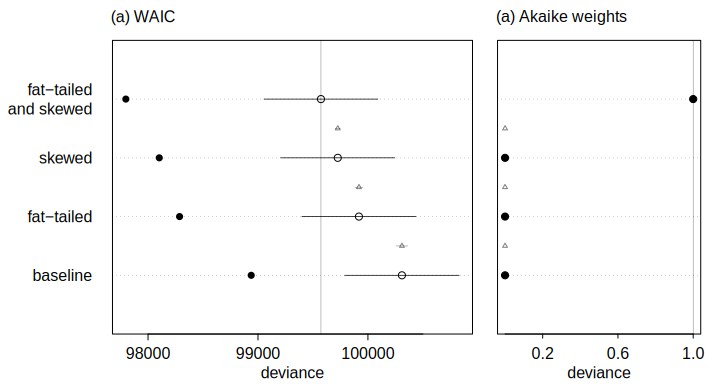
\includegraphics[width=0.8\textwidth]{figures/WAIC-plot}
    	  \vspace{0.3cm}
	   \caption{Comparison of the different models using WAIC values. Each row describes one of the models described in the main text. (a) WAIC comparison of the different models. The filled points are the in-sample deviance of each model, and the open points are the estimated WAIC values. The dark line segments represent the standard error of each WAIC. The standard error of the difference between each WAIC and the best performing model (top row) is characterized by the gray triangles and line segments. The vertical line references the model with the lowest WAIC value. (b) Akaike weight for each model used to compare predictive accuracy of the different Bayesian models (see \citealt{mcelreathStatisticalRethinkingBayesian2020}). According to this measure, the model with fat-tails and skewed response is the best model. The open points are the mean Akaike weights and the line segments represent the corresponding standard error. The vertical line references the model with the highest Akaike weight. These graphs were generated using some of the functions from the R package \textit{rethinking} \citep{mcelreathStatisticalRethinkingBayesian2020}.}
      \label{sfig:WAIC}
\end{figure}

\clearpage

\begin{figure}[h]
  \centering
    \vspace{0.5cm}
    \includegraphics[width=0.8\textwidth]{figures/nu-kurtosis}
    	  \vspace{0.3cm}
	   \caption{Variability in the tails.}
      \label{sfig:nu-kurtosis}
\end{figure}

\clearpage

\section*{Supplementary Tables}

\begin{table}[h]
\begin{center}
\begin{tabular}{ p{8em} p{6em} l p{16em}} 
\textbf{Information} & \textbf{Variable type} & \textbf{Variable} & \textbf{Description} \\
\hline
\multirow{3}{7em}{ecological indicator values} & \multirow{3}{6em}{climate indicators} & temperature & \textit{10 classes ranging from alpine climates to very warm collines} \\
& & continentality & \textit{5 classes ranging from oceanic to continental climates}\\ 
& & light & \textit{5 classes ranging from deep shade to full light}\\ 
\cline{2-4}
& \multirow{5}{6em}{soil indicators} & moisture & \textit{10 classes ranging from very dry to flooded soil} \\
& & reaction & \textit{5 classes ranging from extremely acid to alkaline soil} \\
& & nutrients & \textit{5 classes ranging from very infertile to over-rich soils} \\ 
& & humus & \textit{5 classes ranging from little to high humus content} \\
& & aeration & \textit{5 classes ranging from bad to good aeration} \\ 
\hline
\multirow{3}{7em}{range of variation} & \multirow{3}{6em}{climate indicators} & temperature & \multirow{3}{14em}{\textit{3 classes indicating small, large and unlimited variation of the different climatic indicators}} \\  
& & continentality & \\ 
& & light & \\ 
\cline{2-4}
& \multirow{3}{6em}{soil indicators} & moisture & \multirow{5}{14em}{\textit{3 classes indicating small, large and unlimited variation of the different soil indicators}}  \\ 
& & reaction & \\ 
& & nutrients & \\ 
& & humus & \\ 
& & aeration & \\ 
\hline
\multirow{3}{7em}{species types} & \multirow{2}{6em}{time of immigration} & invasion status & \textit{classified as indigenous, historical range expanders and recent range expanders} \\  
& \makecell[l]{ \\change\\tendency} & abundance & \textit{classified as stable, decreasing, decreasing at low elevations, and increasing in abundance}\\ 
\hline  
\end{tabular}
\end{center}
\caption{Indicator values \citep{landoltFloraIndicativaOkologische2010}}
\label{stab:EI}   
\end{table}

\begin{table}[h]
\begin{center}
\begin{tabular}{  p{6em} | p{1em} l l } 
\textbf{response curve} & &  \(\beta^{\prime}_i\) & \(\gamma^{\prime}_i\) \\
\\[-1em]
\hline
\\[-1em]
baseline & & \(\beta_i\) & \(\gamma_i\) \\
\\[-1em]

\\[-1em]
fat-tailed & & \(\beta_i\) & \( g = \sqrt{\frac{\gamma_i \Gamma\left(\frac{3}{\nu_i}\right)}{\Gamma\left(\frac{1}{\nu_i}\right)}}\) \\
\\[-1em]

\\[-1em]
skewed &  & \( q_2 = \beta_i - \frac{2 \lambda_i}{\sqrt{\pi} \gamma^{\prime}_i}  \)  & \( q_1 = \gamma_i  \sqrt{\frac{\pi\left(1+3 \lambda^{2}_{i}\right)-8\lambda^2_i}{2\pi}}  \)  \\
\\[-1em]
  
\\[-1em]
\multirow{-1.25}{6em}{skewed and fat-tailed} & & \( f_2 = \beta_i - \frac{2^{\frac{2}{\nu_i}}\lambda_i \Gamma\left(\frac{1}{2}+\frac{1}{\nu_i}\right)}{\sqrt{\pi}\gamma^{\prime}_i}   \)  & \( f_1 = \gamma_i \sqrt{\frac{\pi \left(1+3\lambda^2_i\right) \Gamma\left(\frac{3}{\nu_i}\right)-16^{\frac{1}{\nu_i}} \lambda^{2}_{i} \Gamma\left(\frac{1}{2}+\frac{1}{\nu_i}\right)^2 \Gamma\left(\frac{1}{\nu_i}\right)}{\pi \Gamma\left(\frac{1}{\nu_i}\right)}} \) \\
\\[-1em]
  
\end{tabular}
\end{center}
\caption{cite vignette}
\label{stab:formulas}   
\end{table}


\bibliography{references2}

\end{document}
